\documentclass[twoside,12pt]{article}

\usepackage[nottoc,numbib]{tocbibind}

\usepackage{amsmath,amsfonts,amsthm,fullpage}
\usepackage{amsmath}
\usepackage{amssymb}
\usepackage{listings}
\setlength{\parindent}{0pt}
\usepackage{graphicx}
\usepackage{bm}
\usepackage[section]{placeins}

% Use the standard article template.
%
% The geometry package allows for easy page formatting.
\usepackage{geometry}
\geometry{letterpaper}
% Load up special logo commands.
\usepackage{doc}
% Package for formatting URLs.
\usepackage{url}
% Packages and definitions for graphics files.
\usepackage{epstopdf}
\DeclareGraphicsRule{.tif}{png}{.png}{`convert #1 `dirname #1`/`basename #1 .tif`.png}

\def\argmin{\operatornamewithlimits{arg\, min}}
\newcommand{\rbr}[1]{\left(#1\right)}
\newcommand{\cbr}[1]{\left\{#1\right\}}
\newcommand{\Ncal}{\mathcal{N}}

\renewcommand{\familydefault}{\sfdefault}

%
% Set the title, author, and date.
%
\title{Yelp - Personalized Restaurant Recommendation}
\author{Ajay D'Souza (adsouza31)}
\author{
  D'Souza, Ajay\\
  \texttt{ajaydsouza@gatech.edu}
}
\date{}
  
\iffalse
*------------------------------------------------------------*
  These are the instructions from Polo for the Final Report
*------------------------------------------------------------*
Final Report
It will be a detailed description of what you did, what results you obtained, and what you have learned and/or can conclude from your work.

Components:

Writeup: fewer than 2800 words, 12pt font, typed. Describe in depth the novelties of your approach and your discoveries/insights/experiments, etc.  
Software: packaging, documentation, and portability. The goal is to provide enough material, so that other people can use it and continue your work.
Grading scheme & Submission instructions
Writeup
[2%] Introduction - Motivation
[3%] Problem definition
[5%] Survey
Proposed method
[10%] Intuition - why should it be better than the state of the art?
[35%] Description of your approaches: algorithms, user interfaces, etc.
Experiments/ Evaluation
[5%] Description of your testbed; list of questions your experiments are designed to answer
[25%] Details of the experiments; observations (as many as you can!)
[5%] Conclusions and discussion
[-5% if not included] Distribution of team member effort. Can be as simple as "all team member contribute similar amount of effort". If effort distribution is too uneven, I may assign higher scores to members who contributed more.
Team's contact person submits one zip file, via T-Square, that contains the following (software + writeup softcopy) [10%]:
a concise, short README.txt file, corresponding to the "user's manual". This file should describe the package in a few paragraphs, how to install it, how to use it, and how to run a demo.
a folder called DOC (short for "documentation"), which contains
your report write up in PDF format (can be created using any software, e.g., latex, Word), named teamXXreport.pdf, via T-Square, where XX is the team number (e.g., team01report.pdf for team 1)
any files related to your final (poster) presentation (e.g., PDF of your final poster)
make sure that your package includes only the absolutely necessary set of files!
\fi

\begin{document}

\maketitle
\begin{center}

\includegraphics{logo.png}
\end{center}

% Add an abstract.
\begin{abstract}
\textbf{Datatouille} - Personalized Restaurant Recommendation using Yelp reviews : \\
Mine Yelp restaurant reviews to extract the dish names a user likes in a restaurant. Use these dish names to recommend new dishes along with specific restaurants that specialize in those dishes.
\end{abstract}
% Add various lists on new pages.
\pagebreak
\tableofcontents

\pagebreak
\listoffigures
\listoftables

% Start the paper on a new page.
\pagebreak



%
% Body text.
%
\section{Introduction}
\label{Introduction}
Currently when recommendation systems recommend restaurants to users using a star rating, the dish names that appeal to a users palate generally remain as unlabeled latent features in that recommendation in the currently popular matrix factorization family of algorithms.\footnote{Heilmeier Question No.2}\\

The goal of this project is to be able to understand user tastes and recommend to the user one or more specific dishes, followed by a recommendation of restaurants in the users geographic neighborhood that specialize in those dishes \footnote{Heilmeier Question No.1}. We want to expose dish name which is central to restaurant recommendation as a labelled feature in our recommendation system.\footnote{Heilmeier Question No.3}



\section{Problem Definition}
\label{Problem Definition}
Choosing a restaurant is a very personal choice. Using star ratings does not provide a personalized basis for recommendation. The Yelp Challenge dataset provides close to a million tuples of (user, restaurant, timestamp, review). From the reviews in each tuple we will extract the dish names. If the User has mentioned a dish we assume the user likes the dish. \textit{Like} and \textit{dislike} will be stored as binary values. Next, if the user expresses a positive sentiment of the experience of having that dish in that particular restaurant,  we assume that the restaurant \textit{specializes} in that dish.
We keep a count of the number of users expressing positive sentiment for a dish-restaurant tuple as a measure of the restaurant specializing in that dish.\\

We build a sparse table $User \times Dish$. We perform Item Based Collaborative Filtering and User Based Collaborative Filtering to generate  \textit{top-N} recommendations of dishname and restaurant specializing in these dishes for a given user. Results will be filtered by the geographic location of the user.


\section{Survey}
\label{Survey}

\subsection{Dish name Extraction}

\cite{andrew_scott} presents a hybrid approach where a gazetteer-driven NER algorithm is used to partially label the corpus. The partially labeled corpus is then used to train a sequence model that induces labels on the remaining entities.\\

\cite{ritter_clark} discusses the degradation of performance of NLP tools when applied to social media. It discusses the POS tag patterns that can be used to get named entities.\\

\cite{lafferty_2001} was studied while evaluating CRF approach in  \cite{tzonghan} for Random Forests based classification. \\

\cite{robin_jean} was studied to understand the variable importance feature in Random Forests.


\subsection{Sentiment Detection}

\cite{pang_2002} discusses the methods of Naive Bayes (NB), SVM and Max Entropy(MAXENT) for sentiment detection of movie reviews. The authors build a labeled vocabulary of uni-grams and bi-grams from the corpus of labeled movie reviews. Classifiers are trained using this  vocabulary. The NB, SVM and MAXENT classifiers reported comparable accuracy of around $80\%$ with the test data\\

\cite{das_2001} specifies a way to handle negation words by appending  NOT\_ to every word between the word with negation till the next punctuation mark. Using this approach words like $isn't good$ will get negation tags and are likely to be seen as negative as they should be.\\

\cite{turney_2002} and \cite{turney_littman_2002} provide a unsupervised method for sentiment classification. The method picks the adjective and adverb phrases from the POS tag patterns shown in table $\eqref{PMI Phrases}$ below.\\ 

\begin{table}[ht]
\centering
\resizebox{\textwidth}{!}{
\begin{tabular}  {| c | c | c | c |}
 \hline
 & First Word & Second Word & Third Word (Not Extracted)\\
 \hline
1.& JJ & NN or NNS & anything\\
\hline
2.& RB, RBR, or RBS & JJ  & not NN nor NNS\\
\hline
3.& JJ & JJ & not NN nor NNS \\
\hline
4.& NN or NNS & JJ & not NN nor NNS \\
\hline
5.& RB, RBR, or RBS & VB, VBD, VBN, or VBG & anything \\
 \hline
\end{tabular}}
\caption{Phrases to be extracted for PMI}
\label{PMI Phrases}
\end{table} 

It then performs a web search to compute their Pointwise Mutual Information (PMI) score as in $\eqref{pmi}$, and the Semantic Orientation as shown in $\eqref{pmi_so}$. The review is taken to be positive if the average SO of all the phrases in a review is positive. 

\begin{align}
PMI(word_1, word_2) &= \log_2 \left(\frac{p(word_1 \&\, word_2)}{p(word_1) p(word_2)}\right) \label{pmi}\\
\nonumber\\
SO(phrase) &= PMI(phrase, “excellent”) - PMI(phrase, “poor”) \label{pmi_so}
\end{align}

\subsection{Recommender Systems}
\cite{yehuda_matrix_factorization} discusses the NMF matrix factorization method for recommender systems. For sparse matrices and for serial computation Stochastic Gradient Descent is recommended as an suitable choice.

\cite{funk_matrix_factorization} details the implementation of the Stochastic Gradient Descent method for matrix factorization.

\cite{cf_online}  describes how Item Based and User Based Collaborative Filtering can be used to determine similarities between items' consumption and user consumption respectively. It also explains how to make a recommendation using this two approaches.

\section{Intuition}
\label{Inuition}
The state-of-the-art in restaurant recommendation systems is to base recommendations on star ratings made by all users, which can leave out significant details such as restaurant specialty and user preference. Since Datatouille uses a user's own reviews to understand which dishes a user likes and a restaurant's reviews to determine the restaurants specialty, a recommendation can more accurately pair a user with a restaurant and make a truly personalized recommendation\footnote{Heilmeier Question No.3 - Why it will be successful ?}.

\section{Proposed Method}
\label{Proposed Method}

The following figure gives a high level overview of the different components of Datatouille:
\begin{figure}[ht]
  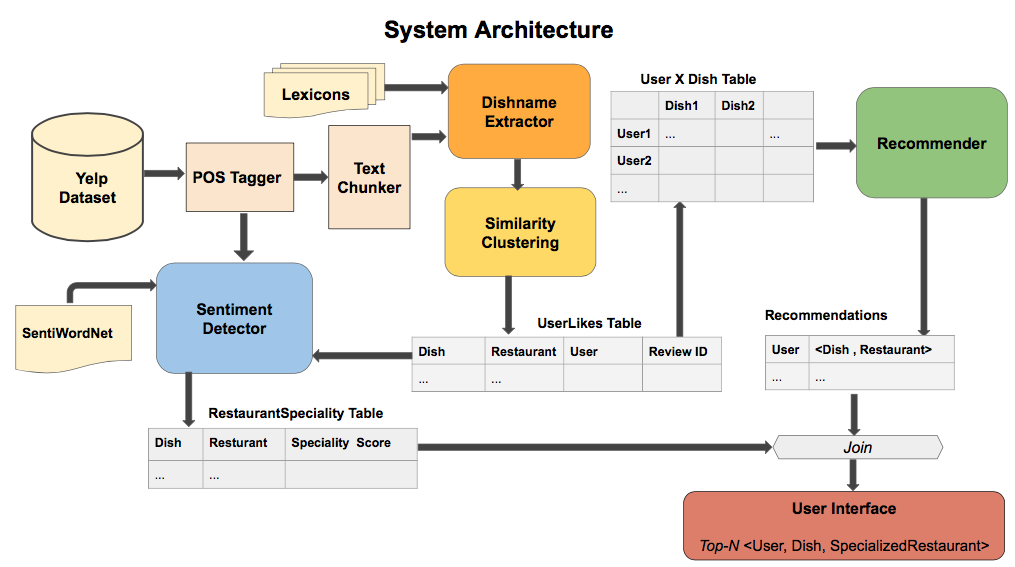
\includegraphics[width=\textwidth]{systemArch.png}	
  \caption{Components of Datatouille}
\end{figure}

\subsection{DishName Extraction}
We use Random Forests classifier as below \cite{ritter_clark}. 

\begin{enumerate}
\item
Label Data

From a mix of reviews we generate a set of 9500 n-grams (n = 2 to 6). The n-grams are labeled as either DISHNAME or NOT\_DISHNAME. We divide these into a test set of 1500 items and training set of 8000 items.

\item
We POS tag each sentence as in figure \ref{fig:dish_name_extraction_pos_tagged_sentence}

E.g. For sentence "I ordered Buddha Spring Roll and chicken fried rice", we get

\begin{figure}[ht]
  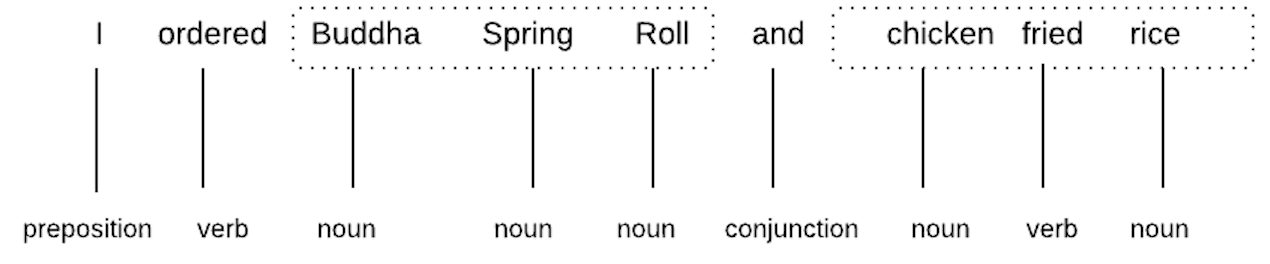
\includegraphics[width=\textwidth]{pos1.png}	
  \caption{Dish Name Extraction - POS Tagged Sentence }
  \label{fig:dish_name_extraction_pos_tagged_sentence}
\end{figure}


\item
Text is chunked, relevant n-grams in noun phrases and  n-grams outside noun phrases are extracted as shown in figure \ref{fig:dish_name_extraction_n_grams}.

\begin{figure}[ht]
  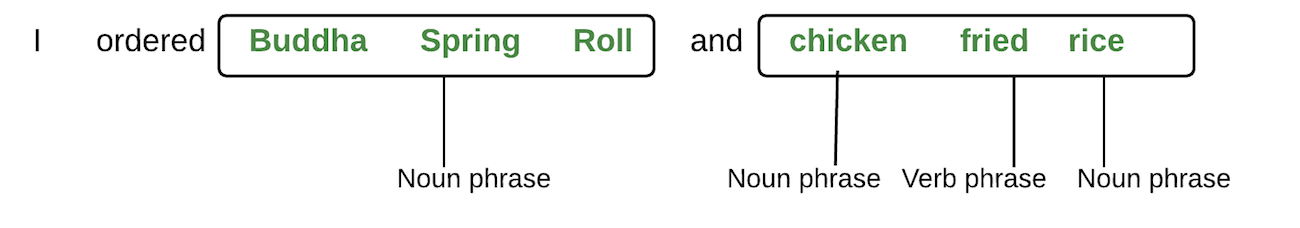
\includegraphics[width=\textwidth]{pos3.png}	
  \caption{Dish Name Extraction - n-grams}
  \label{fig:dish_name_extraction_n_grams}
\end{figure}


\item
Food lexicons were created using readily available information on the web, we  generate the following boolean feature vector for each selected n-gram.

\begin{enumerate}
\item
Begins with Noun ?
\item
Begins with \textit{relevant adjectives} that commonly appear in food names ? E.g.: spicy
\item
Begins with \textit{relevant verbs} commonly used in Yelp restaurant reviews ? E.g. ordered.
\item
Ends in Noun ?
\item
Has a food context clue ?. This is guessed from the presence of  \textit{cooking style} terms. E.g. fried,  \textit{Common Food} nouns E.g. Pizza and \textit{relevant adjectives} in the n-gram
\item
All words in a noun phrase ?
\item
Is dish name ? (training label)
\end{enumerate}


\item
Random Forests with the following parameters was used to train the classification model
\begin{enumerate}
\item
Number of trees: 10
\item
Quality of split function: Gini
\item
Maximum features: Square root of number of features
\end{enumerate}

\end{enumerate}

\subsection{Similarity Clustering}
The dish names from different reviews may differ due to spelling errors, use of short names (substring of the main name). Levenshtein distance is used to find similar dish names. A graph of similar dish names as adjacent nodes is created. The graph is sorted by node degree and clusters of  one hop neighbors are created. Each cluster represents a single dish entity.

\subsection{Sentiment Detection}
We chose to use Naive Bayes (NB) classifier for sentiment detection, since a large domain specific corpus is available for training it. Levenshtein distance is used to determine similar dish names and a graph of dish names with similar names is created.

\begin{enumerate}
\item
Manually labeled 3000 random sentences as positive, negative or neutral on sentiment. This is the test set for measuring classifier performance.
\item
From the proportion of labels in the training data compute the class priors. For training, we use the overall rating as the class label. A rating of $4,5$ is taken as positive, $3$ as neutral and $1, 2$ as negative.
\item
POS tag each review sentence, remove stop words and nouns
\item
Use NOT\_ as the negation tag on every word between the negated word and the next punctuation
\item
Build an effective vocabulary of uni-grams and bi-grams to build a feature vector.
\item
Train the NB classifier by calculating the probability of each uni-gram or bi-gram in the feature vector with Laplace smoothing as
\begin{align}
P(w_i|c_j) &= \frac{ count(w_i \in c_j) + 1}{\sum_i count(w_i \in c_j) + |V|+1} \label{nb_p1}\\
|V| &= \text{size of the vocabulary used}
\end{align} 
\item
Additional features where engineered for the following factors 
\begin{enumerate}
\item
Overall rating provided by the user 
\item
sentiment polarity for words in the $SentiWordNet$ lexicon
\end{enumerate}
With the trained NB model we can classify a sentence as below
\begin{enumerate}
\item
Tokenize the sentence to be classified. Construct a binary array for presence of n-grams in the feature vector of the trained NB classifier.
\item
Compute the probability of a sentence belonging to a class as
\begin{align}
C \gets \underset{j}{\arg max} P(c_j) \prod_{i} P(w_i|c_j) \label{nb_p2}	
\end{align}
\end{enumerate}
\end{enumerate}


\subsection{Recommendation Engine}

We employ the following algorithm similar to \cite{cf_online} for Datatouille recommendations.
\begin{enumerate}
\item
A $User \times Dish$  table is given as input. Create a \textit{Dish} table by dropping the \textit{User} column.
\item
Perform Item Based CF: 

A $Dish \times Dish$  similarity matrix is formed using \textit{Cosine similarities} between the dish vectors from the \textit{Dish}    table. 
\item
Perform User Based recommendation:

Create the $User \times Dish$   \textit{Recommendation Matrix} where every entry has a score calculated thus:

For every user U and every dish D that user has consumed:
\begin{enumerate}
\item
Identify \textit{Top-N} similar dishes of D from $Dish \times Dish$  similarity matrix and get similarity scores in $d_s$ vector.  
\item
Get a consumption record as  ${c_r}$  vector of the user U from  $User \times Dish$  for each of the similar dishes.
\item
For each similar dish, ${Score_{u,d}}$ =   $\frac{d_s^{T}  . c_r}{L1 Norm (d_s)}$ is calculated and updated in the matrix at ${(u,d)}$
\end{enumerate}
\item
For a given user, we identify a row in $User \times Dish$  \textit{Recommendation Matrix} , we return Top-N dishes by sorting the values of the user row.
\end{enumerate}

\subsection{User Interface}
UI is through a web interface. For a chosen user it displays the name of the restaurant along with the dishes recommended. The display is on a interactive map with marker sizes showing the strength of the recommendation.


\subsubsection{Data Visualization}
We intend to have visualization of aspects of algorithm for data extraction and the sentiment detection. 


\subsection{Innovation}
\begin{enumerate}
\item We demonstrate how to choose and use labeled features with existing recommendation algorithms for deriving relevant recommendations instead of a star rating. This idea can also be extended to algorithms that uses matrix factorization with star ratings where important features remain latent with no control over them.
\item 
For sentiment detection we used an ensemble of NB classifier based on corpus vocabulary and the average Sentiment Orientation of a sentence based on sentiment polarity of sentiment expressing words from SentiWordNet.
\item
Use a combination of NLP and online lexicons to train a simple Random Forest classifier using a smaller corpus of training data for extracting dish names.
\end{enumerate}


\subsection{Implementation Details}

\subsubsection{Dish Name Extraction}
Feature vector generation for dish name extraction is implemented in Java using Stanford POS and Apache OpenNLP libraries. The classification algorithm is implemented in Python using scikit-learn's RandomForestClassifier.

\subsubsection{Sentiment Detection}
Sentiment detection is implemented using python. The python nltk module is used for tokenizing, POS tagging and stop word removal. The $SentiWordNet$  lexicon is used for sentiment polarity. The classifier was trained using ten fold cross validation. A labeled data set of 3000 reviews was used for testing.

\subsubsection{Recommendation Engine}
The recommendation engine is built as detailed in proposal section using python along with the pandas and scipy library. The pandas library assisted in keeping track of data while the scipy library provided a function to compute cosine similarities.

\subsection{UI}
The UI pulls together the original Yelp dataset for information about users and businesses with the recommended dishes and restaurants for a user and displays the information on Google Maps. 

\begin{figure}[hb]
	\centering
	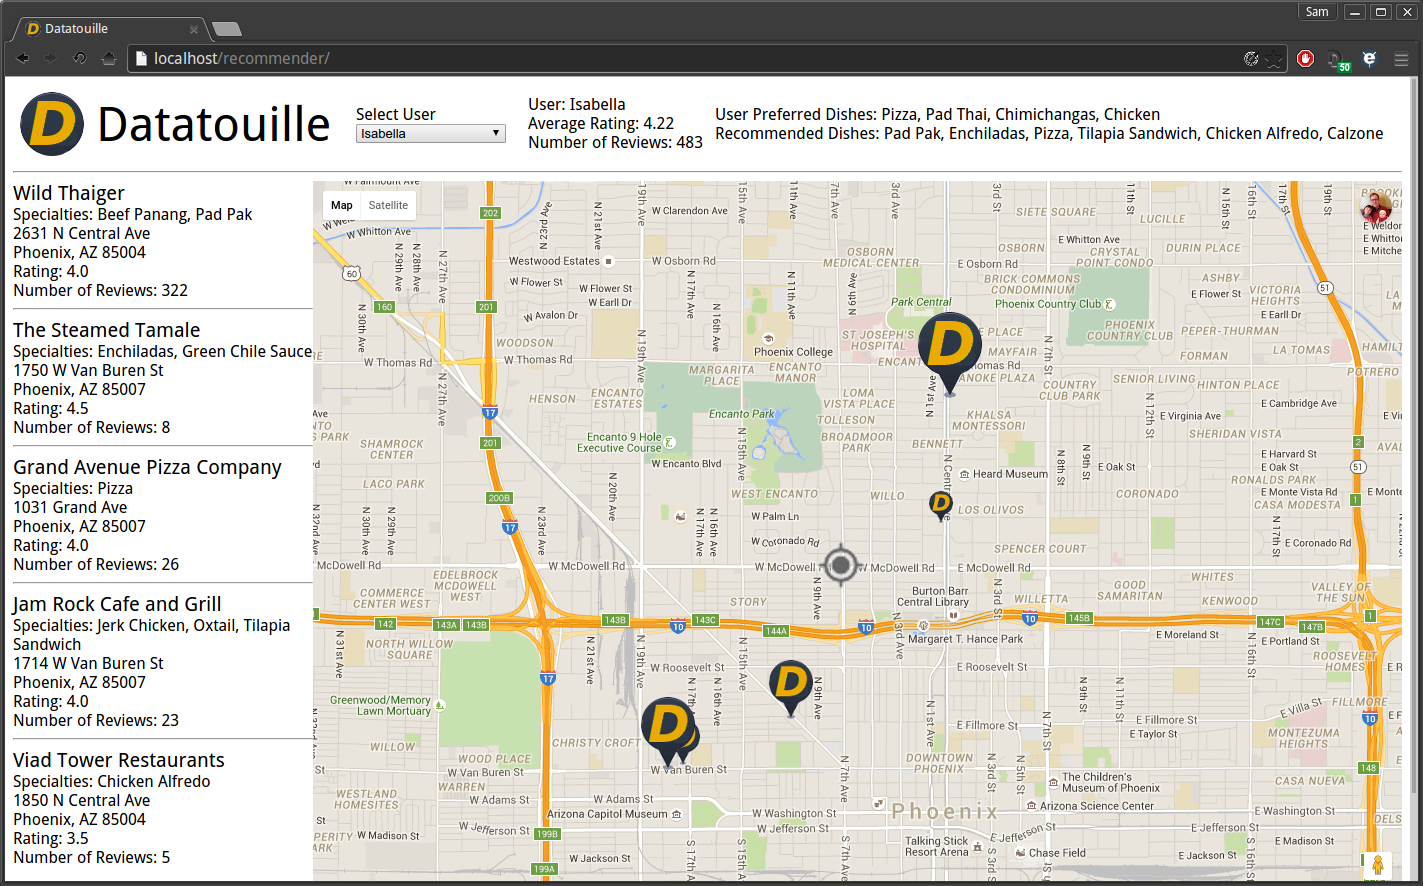
\includegraphics[width=100mm]{screenshot.png}
    \caption{Datatouille UI}
\end{figure}

For the demo, select a user from the combo box. The user's Yelp information will be displayed at the top of the page alongside the dishes extracted from the user's reviews and a list of suggested dishes. The recommended dishes are used in a query on the table of restaurant specialties. For portability, sqlite was used as the database back end, but it lacks the math functions (sin and cos) required to calculate the distance from the user's current location to the restaurant. With a more robust database solution, the final goal can be fully realized. 

\section{Experiments and Evaluation}
\label{Experiments and Evaluation}
Dish name extraction accuracy was measured for precision and recall on a labeled test data set  1500 labeled sentences
\newline

Sentiment detection accuracy was measured on a labeled test data set of 3000 labeled sentences.
\newline

For measuring performance of recommender system we propose to use reviews of a subset of users as the test set. We will use their reviews up to some point in time $t_1$ to make a recommendations. We will then measure the recommendations made with the actual restaurants reviewed by the same user after that point in time $t_1$
\newline

Dish name extraction was evaluated using Google-Refine which first yielded roughly 87,000 different dishes for the Phoenix area. Google-Refine's cluster feature provided a way to see if top clusters were dishes or not. 
\newline

The data was then filtered when building the $User \times Dish$  to only include the dishes that occurred 50 times or more, this left 688 dishes. After a manual review it was found that only  6.98\%  were terms that did not correspond to dishes; these dishes were omitted from data. 
\newline

Due to paucity of time sentiment detection is not integrated in the UI. Instead of using sentiment detection, the recommendation system uses the presence of a dish in the dish extraction as an indication of user preference and restaurant specialty.
\newline

To test the UI, several users were chosen from the drop down box. Their dish recommendations were compared to the extracted dishes for consistency. The restaurant recommendations were confirmed based on the results. The best test of the UI and the entire project as a whole would be to let numerous people try the project and record their experiences with a questionnaire. Time did not permit this.
\newline

Recommendation was verified manually while testing the UI. The sample below shows how relevant dishes are recommended to a used based on preferred dishes. In this example Matthew likes Fish Tacos and only taco related items are recommended. Also, Matthew only has one preferred dish because he only has two reviews so only one dish was extracted for that user. 
\newline

\begin{figure}[ht]
	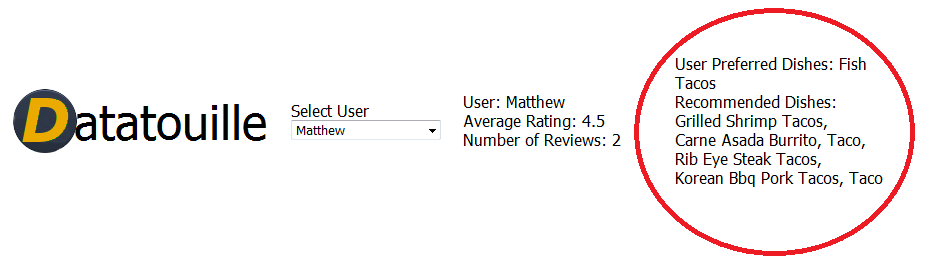
\includegraphics[width=\textwidth]{MatthewTacoRecomend.png}
    \caption{Sample Recommendation from UI}
\end{figure}


\section{Results and Observations}
\label{Results and Observations}
The following results where observed \footnote{Heilmeier Question No. 9}
\begin{itemize}
\item
Performing Principal Component Analysis using these feature vectors generated for dish name extraction shows separation of the DISHNAME and NOT\_DISHNAME labeled training data $\eqref{pca_dish_name_extraction}$, thus providing a validation for the features engineered. 

\begin{figure}[ht]
   \centering
   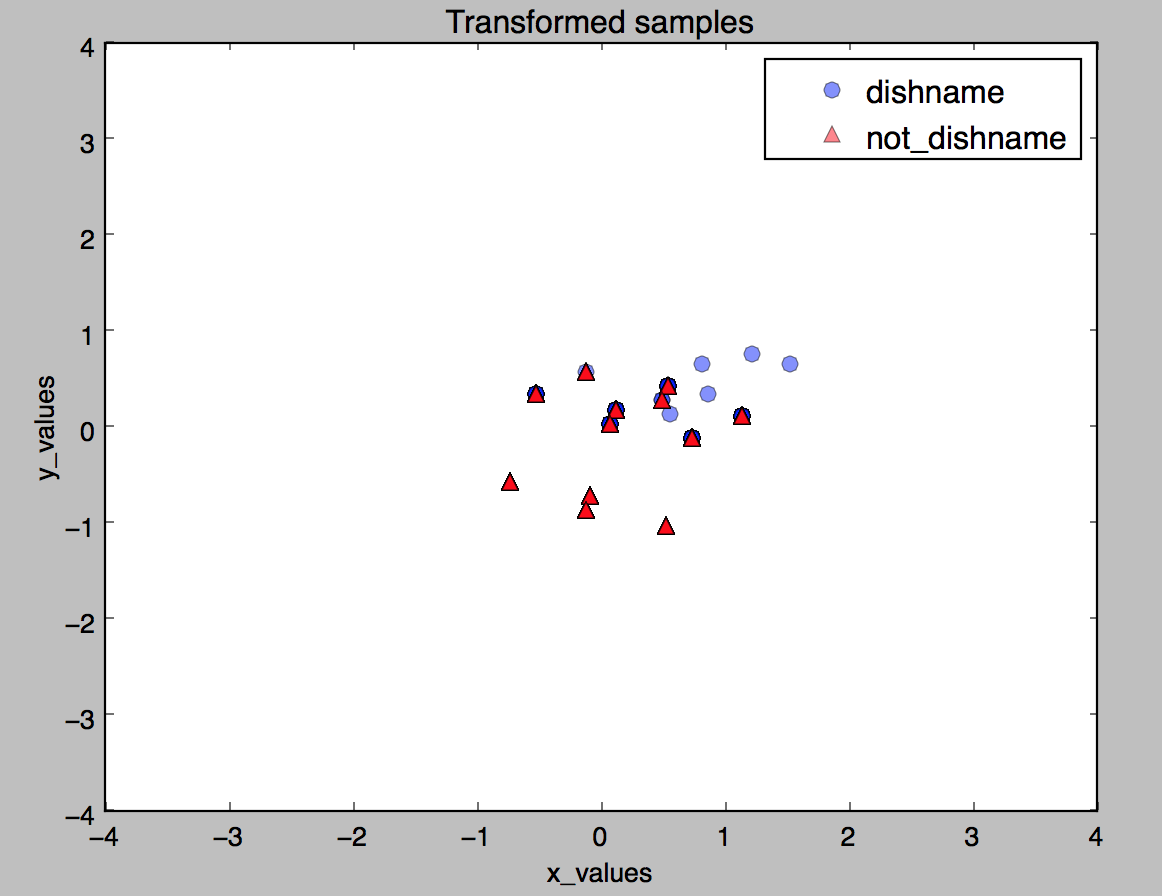
\includegraphics[width=100mm]{pca.png}	
  \caption{Dish Name Extraction - PCA}
  	\label{pca_dish_name_extraction}
\end{figure}

\item
The ROC plot for the classification model created with $1500$ test n-grams is shown in figure $\eqref{dish_name_extraction_roc_plot}$ below. A prediction probability$\ge$ 0.8 is chosen.

\begin{figure}[ht]
   \centering	
   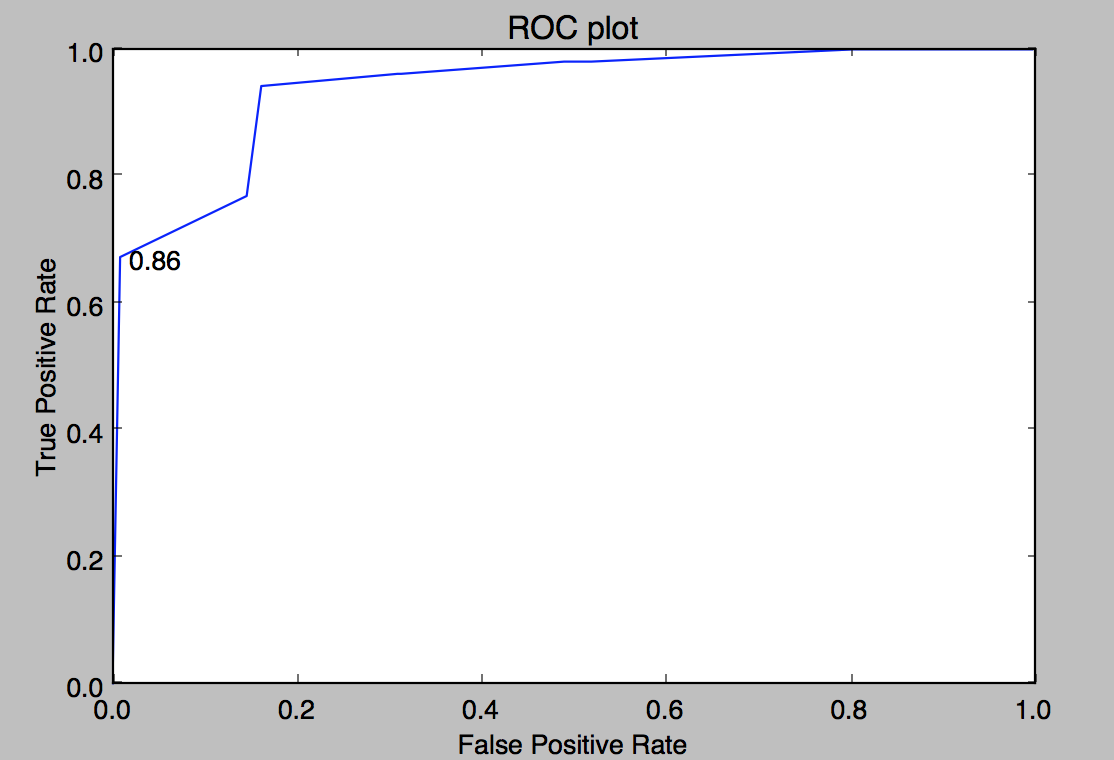
\includegraphics[width=100mm]{roc.png}	
  \caption{Dish Name Extraction - ROC plot}
  \label{dish_name_extraction_roc_plot}
\end{figure}

\item
The confusion matrix for dish name extraction based on a 1500 n-grams labeled test data is below $\eqref{dish_name_extraction_confusion}$.  Precision: $76\%$ and Recall: $71\%$ 

\begin{figure}[hb]
  \centering
  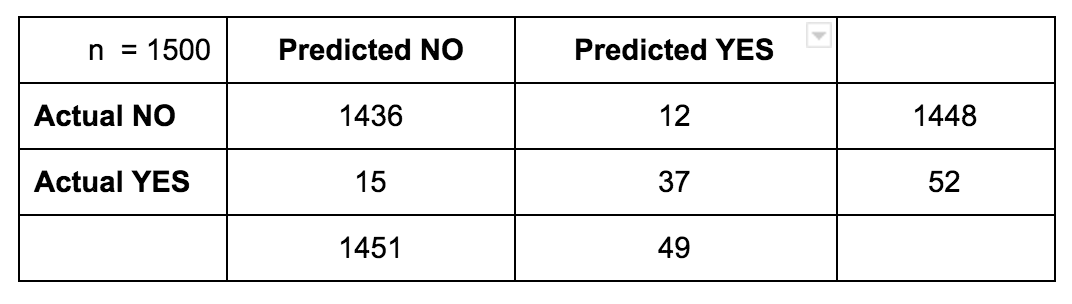
\includegraphics[width=\textwidth]{confuse.png}	
  \caption{Dish Name Extraction - Confusion Matrix}
  \label{dish_name_extraction_confusion}
\end{figure}

\begin{figure}[hb]
	\centering
	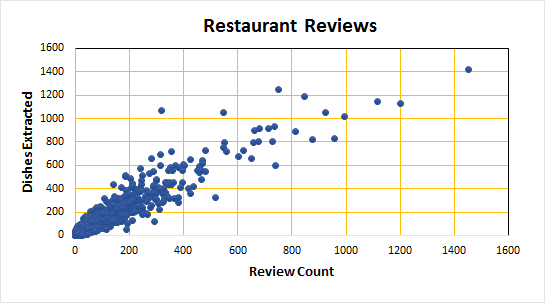
\includegraphics[width=100mm]{restReviewDishesExt.png}
    \caption{Dishes extracted versus review count. Almost a consistent dish per review trend.}
\end{figure}
\item
Sentiment detection was tested on a labeled set of 3000. The Naive Bayes classifier gave an accuracy of $65.67\%$ on this labeled set
\item
$\eqref{confusion_matrix_sentiment_analysis}$ is the confusion matrix generated for the sentiment classifier
\begin{table}[ht]
\centering
\resizebox{\textwidth}{!}{
\begin{tabular}  {| c | c | c | c | c |}
\hline
 & Predicted Positive & Predicted Neutral & Predicted Negative &  Total \\
\hline
 Actual Positive & 1146 & 345 & 77 & 1568\\
\hline
 Actual Neutral & 186 & 382  & 76 & 644 \\
\hline
 Actual Negative & 67  & 282 & 439 & 788 \\
\hline
  Total & 1399  & 1009  & 592 & \\
 \hline
\end{tabular}}
\caption{Confusion Matrix for Sentiment Detection}
\label{confusion_matrix_sentiment_analysis}
\end{table} 
\item
$\eqref{precision_recall_matrix_sentiment_analysis}$ is the Precison and Recall table for the sentiment detection. The tests showed the best precision and recall for the positive class. This serves the projects requirement as we are interested only in reviews which are positive. 
\begin{table}[ht]
\tiny
\centering
\resizebox{\textwidth}{!}{
\begin{tabular}  {| c | c | c |}
\hline
 Class & Precision(\%) & Recall (\%) \\
\hline
 Positive & 81.92 & 73.08 \\
\hline
 Neutral & 37.85 & 59.32 \\
\hline
 Negative & 74.15  & 55.71  \\
\hline
\end{tabular}}
\caption{Precision Recall Matrix for Sentiment Detection}
\label{precision_recall_matrix_sentiment_analysis}
\end{table}
\item
Due to paucity of time Sentiment detection module is not integrated with the UI. However these test results indicate that it will integrate well with the UI and enhance user experience.
\item  
The $User \times Dish$  matrix is sparse but shows adequate overlap of different users and different dishes. This implies good recommendation model using this matrix is possible. A 1000 x 800 segment of the original matrix is shown here.
\begin{figure}[hb]
	\centering
	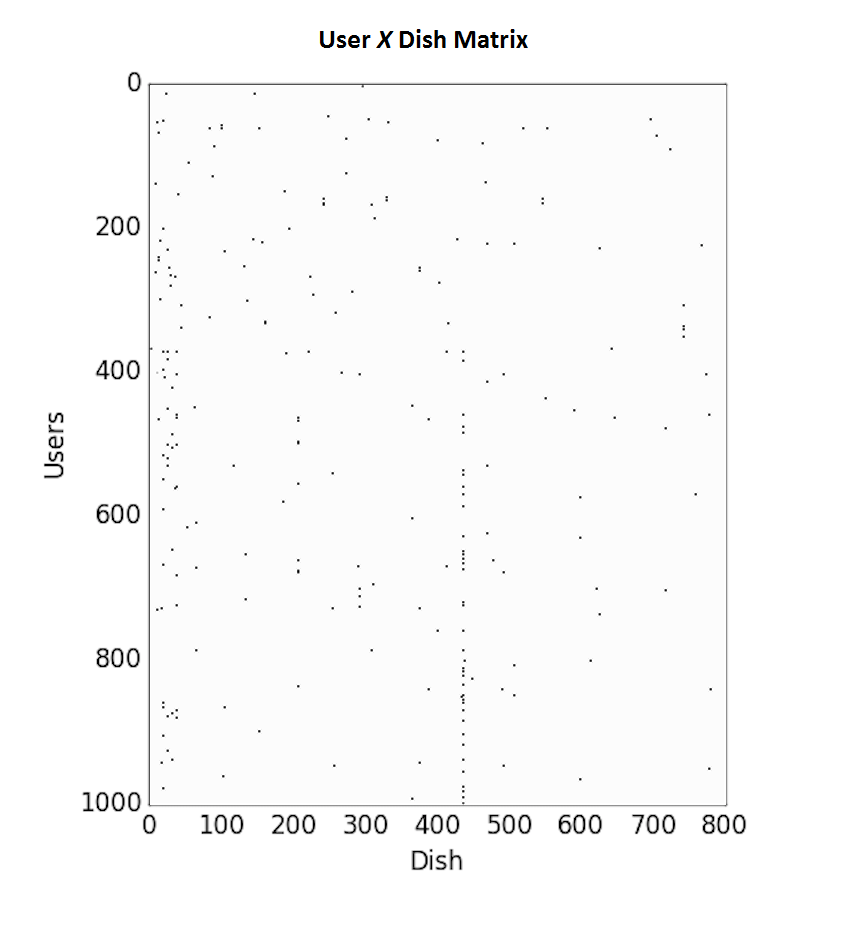
\includegraphics[width=100mm]{sparse.png}
    \caption{User X Dish Matrix.}
\end{figure}
\item Recommender system chose dishes within a high degree of similarity to the user's reviewed dishes. 
\end{itemize}


\section{Conclusions}
\label{Conclusions}
\begin{itemize}
\item
Using the dishes a user has reviewed as a basis for recommending a restaurant provides a personalized method for bringing in customers. With dish extraction and sentiment analysis, the preferences of a user and the specialties of a restaurant can be mined from a dataset of user reviews. Dish and restaurant recommendations can be produced that match a user's tastes and presented to the user in an intuitive manner \footnote{Heilmeier Question No.4}.
\item
The quality of recommendations made can be further improved by using an ensemble of classifiers which use POS tags and sentiment lexicon knowledge as well. We believe that a effective way to judge the efficacy of our approach is to compare it with the recommendations from a $User \times Dish$ matrix. This will reveal if using explicit features enhances accuracy over relying latent features.
\item
This approach can be applied to other domains as well, where explicit features from review content can be used to enahance recommendation accuracy.\footnote{Heilmeier Question No.5}
\item
While the review data is rich in information, any approach that seeks to mine it needs to have domain specific knowledge built into it to improve its tractability for maching learning purposes\footnote{Heilmeier Question No.6}.
\item
The project was implemeted in around 9 weeks using 4 developers. Primarily open source software was used for implementation \footnote{Heilmeier Question No.7 and 8}.
\end{itemize}


%\addcontentsline{toc}{section}{References}
\bibliographystyle{plain}
% Generate the bibliography.
\begin{thebibliography}{9}

\bibitem{ekstrand_2011}
  Michael D. Ekstrand, John T. Riedl.,
  \emph{Collaborative Filtering Recommender Systems},
  Foundations and Trends in Human–Computer Interaction Vol. 4,
  2011.

\bibitem{pazzini_2007}
  M. J. Pazzani, D. Billsus,,
  \emph{Content­Based Recommendation Systems},
  2007.

\bibitem{basu_1998}
  C. Basu, H. Hirsh, W. Cohen,
  \emph{Recommendation as Classification: Using Social and 
  Content­Based information in Recommendation},
  1998.

\bibitem{hajas_2014}
  Peter Hajas, Louis Gutierrez, Mukkai S. Krishnamoorthy,
  \emph{Analysis of Yelp Reviews},
  2014.

\bibitem{slocum_2001}
  Terry A. Slocum, Connie Blok, Bin Jiang, Alexandra Koussoulakou, Daniel R. Montello, Sven Fuhrmann, Nicholas R. Hedley,
  \emph{Cognitive and Usability Issues in Geovisualization},
  2001.

\bibitem{jurafsky_2014}
  Dan Jurafsky, Victor Chahuneau, Bryan R. Routledge, Noah A. Smith,
  \emph{Narrative framing of consumer sentiment in online restaurant reviews},
  2014.
  
    \bibitem{andrew_scott}
  Andrew Carlson, Scott Gaffney and Flavian Vasile.
   \emph{Learning a Named Entity Tagger from Gazetteers with the Partial Perceptron},
   Carnegie Mellon University,
   Yahoo! Labs

    \bibitem{ritter_clark}
  Alan Ritter, Sam Clark, Mausam and Oren Etzioni
   \emph{Named Entity Recognition in Tweets: An Experimental Study},
   University of Washington

 \bibitem{tzonghan}
    Richard Tzong­Han Tsai and Chun­Hui Chou.,
    \emph{Extracting Dish Names from Chinese Blog Reviews Using Suffix Arrays and a Multi­Modal CRF Model},
    Department of Computer Science and Engineering Yuan Ze University, 
    Taiwan.
    
  \bibitem{lafferty_2001}
    J. D. Lafferty, A. McCallum, and F. C. N. Pereira,
    \emph{Conditional random fields: Probabilistic models for segmenting and labeling sequence data},
    In Proceedings of the Eighteenth International Conference on Machine Learning,
    Morgan Kaufmann Publishers Inc.,
    2001.

  \bibitem{robin_jean}
    Robin Genuera, Jean-Michel Poggi∗,a,b, Christine Tuleau-Malotc.
    \emph{Variable Selection using Random Forests},
   Universite ́ Paris-Sud 11, France
   Universite ́ Paris 5 Descartes, France
   


  \bibitem{sutton_2012}
   Charles Sutton and Andrew McCallum.
   \emph{An Introduction to Conditional Random Fields. Foundations and Trend in Machine Learning},
   Vol. 4, 
   2012.

  \bibitem{pak}
  Alexander Pak, Patrick Paroubek, 
  \emph{Twitter as a Corpus for Sentiment Analysis and Opinion Mining}, 
  Alexander , 
  Universit ́e de Paris­Sud, 
  Laboratoire LIMSI­CNRS, Bˆatiment 508,
  F­91405 Orsay Cedex, 
  France

  \bibitem{pang_2002}
  Pang, Bo; Lee, Lillian; Vaithyanathan, Shivakumar,
  \emph{Thumbs up? Sentiment Classification using Machine Learning Techniques},
  Proceedings of the Conference on Empirical Methods in Natural Language Processing (EMNLP). pp. 79–86
  2002
  
  \bibitem{dave}
  Kushal Dave, Steve Lawrence, and David M. Pennock.,
  \emph{Mining the peanut gallery: opinion extraction and semantic classification of product reviews.},
  In WWW ’03: Proceedings of the 12th international conference on World Wide Web, pages 519–528, 
  New York, NY, 
  USA.
  2003
  
  \bibitem{turney_2002}
  Turney Peter,
  \emph{Thumbs Up or Thumbs Down? Semantic Orientation Applied to Unsupervised Classification of Reviews },
  Proceedings of the Association for Computational Linguistics. pp. 417–424,
  2002
  
   \bibitem{turney_littman_2002}
    Turney Peter, Littman L Michael,
    \emph{Unsupervised learning of semantic orientation from a  hundred-billion-word corpus},
    Technical Report EGB-1094, National Research Council Canada,
    2002
 
  
  \bibitem{das_2001}
  Das Sanjiv,Chen Mike,
  \emph{Extracting market sentiment from stock message boards.},
  In Proc. of the 8th Asia Pacific Finance Association Annual Conference
  2001
  
  \bibitem{liu_sentiment}
  Liu Bing,
  \emph{Sentiment Analysis and Subjectivity},
  Handbook of Natural Language Processing (Second ed.),
  2010
  
  
  \bibitem{yehuda_matrix_factorization}
  Koran Yehuda, Bell Robert, Volinsky Chris 
  \emph{Matrix Factorization Techniques For Recommender Systems}
  
  \bibitem{funk_matrix_factorization}
  Funk SImon, 
  \emph{Netflix Update: Try This at Home},
  http://sifter.org/~simon/journal/20061211.html.,
  2006 

\bibitem{cf_online}
  Salem Marafi, 
  \emph{Collaborative Filtering},
http://www.salemmarafi.com/code/collaborative-filtering-r/,
  2014 



\end{thebibliography}

\end{document}